% ============================================================
% 5. Results
% ============================================================
\section{Results}
\label{sec:results}

\subsection{Main Comparison: Target Attainment}

Table~\ref{tab:main} reports target attainment for all eight tasks under
the six columns. Three findings stand out. First, the governed
agent achieves \textbf{8/8} under the two primary models and \textbf{4/8}
under each of the two other models (Section~5.4); every verdict is
computed in code, with an evidence chain per criterion and a verifier-passed
audit chain. Second,
the Bayesian optimizer achieves \textbf{3/8}: exactly T1, T4, and T8, the
three tasks whose binding constraint is structural (thickness, porosity,
mass). Its best designs reach energy densities above the governed agent's on
these tasks (e.g., 678 versus 472 Wh/kg on T4), the expected consequence of
an unconstrained thin-electrode search against a margin-balanced design; on
the remaining five tasks it fails on the design target's own criteria: 4C
plating in T2, T3, T5, T6, T7; SEI limits in T2, T6, T7; a catastrophic
$3.44\%$ 5C retention on T3; the 4.1 V plateau unreachable on T6, where
the best design stalls at the NMC811 plateau limit ($4.0065$ V)---a re-run
with the penalizer aligned to the design target's $50\,^\circ$C red line (the
main run hardcoded $60\,^\circ$C) leaves the outcome unchanged: 0/50 trials
attain the design target in either configuration, 30/50 clear the volumetric
criterion alone in the aligned run, and none is simultaneously
plating-free and below the red line; nail penetration triggered on T7. Figure~\ref{fig:bo} shows the BO trajectories: the three structural
tasks climb to attainment, the five material-bottleneck tasks plateau
against penalties no structural parameter can remove. Third, in the tabulated
workflow-free batch---whose tool asymmetry is disclosed in Section~5.5---no
claim survives within the
measurement space: two of its claimed successes (T4, T8) solve the design target
by switching to a lithium-metal cell outside the validated parameter sets,
and its remaining claims fail re-checking against the criteria (Section~5.5). The
tie between the two baselines (three achieved tasks each) with orthogonal
failure modes is the paper's central observation: the bare agent and the
black-box optimizer fail for different, specifiable reasons, and only the
governed agent passes on all eight targets.

Target-margin calibration deserves explicit reporting, since ``8/8''
could otherwise read as loose thresholds. The thresholds are fixed
increments over the anchoring parameter sets' baseline values, not
frontier-tight values (Section~4.1), and all three conditions face
identical targets: any looseness benefits the baselines equally. The
achieved margins show the design targets binding where they are meant to bind:
on six of the eight governed runs the last criterion to clear sits within
$4.5\%$ of its threshold (T6's plateau at $+0.4\%$ and thermal line at
$+0.5\%$; T8's mass at $+0.5\%$; T3's and T5's thermal lines at
$+1.0$--$1.5\%$); the two exceptions are T2's low-temperature retention
($+10.6\%$) and T7's SEI limit ($+15.4\%$). The wide margins concentrate
on the energy-density clauses of the structural tasks ($+41$--$48\%$),
where an unconstrained thin-electrode search overshoots cheaply; the same
mechanism behind the BO's 678 versus 472 Wh/kg on T4, and precisely the
margin the governed designs partially spend on the safety and durability
criteria. Per-criterion margins for all achieved runs are tabulated in the
supplementary materials. The SEI criteria deserve one further disclosure,
because they are the single criterion class whose bridge lever (the
electrode-modification coating scaling the SEI kinetic rate constant) can
move a verdict: T2 shipped a $10^{-4}\times$ rate constant (declared in
the audit as an estimate beyond the bare-ALD literature magnitude), yet the
identical design passes the design target at $10^{-2}\times$ (500.4 nm against
the 550 nm limit, a $9\%$ margin); T6's SEI work is not verdict-bearing;
T7 used no kinetic override (supplementary materials).

The thresholds are author-anchored, and one threshold property should be
stated in advance of the reader's own check: the comparison's direction is
invariant under a uniform perturbation of them. On the five
material-bottleneck tasks the optimizer's failure is ceiling-bound, not
threshold-bound---across all 400 baseline trials, the highest midpoint
voltage any design reaches is 4.0115 V against the 4.1 V target line, and
plating and SEI violations are lever-bound (supplementary materials). On the
three structural tasks the same criteria bind both conditions in parallel:
under a uniform $+5\%$ tightening the optimizer's attained counts fall from
25/34/10 to 0/22/1, while the governed runs' own binding margins
($+2.2\%$/$+4.5\%$/$+0.5\%$ on T1/T4/T8, Appendix~B of the
supplementary materials) fail
under the same tightening on the same tolerance. No $\pm 5\%$ perturbation
inverts the direction of the comparison; the only conceivable inversion
zone---energy-density thresholds above the governed designs' own margins,
$>+40\%$ on the structural tasks---is exactly the region in which the paper
already reports the optimizer's structural-task energy-density superiority.

\begin{figure}[!ht]
\centering
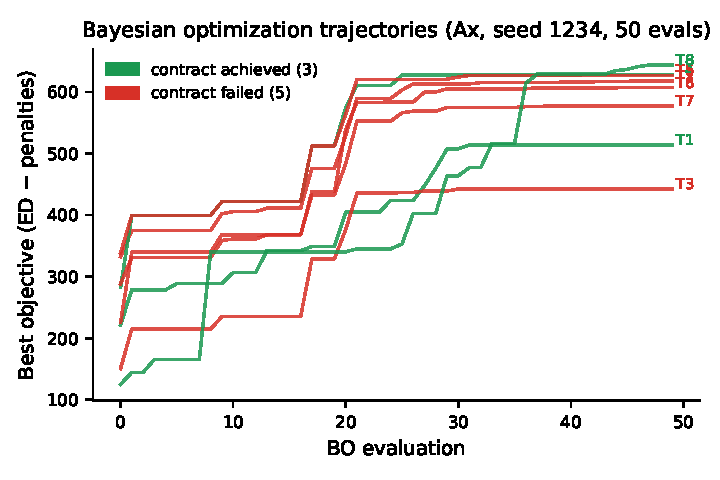
\includegraphics[width=0.8\linewidth]{figs/fig_bo_trajectories.pdf}
\caption{Bayesian optimization best-objective trajectories per task (Ax,
Sobol initialization, GPEI + LogNEI, seed 1234, 50 evaluations). The three
structural tasks (T1/T4/T8) achieve their targets; the five
material-bottleneck tasks plateau against penalties (plating, SEI, plateau,
nail) that no structural parameter can remove.}
\label{fig:bo}
\end{figure}

\begin{table}[!ht]
\centering
\footnotesize
\setlength{\tabcolsep}{3.2pt}
\caption{Target attainment, eight tasks $\times$ six columns
(governed agent shown under four models: pro, flash, luna, mimo).
$\checkmark$ = achieved (code-computed verdict); $\times$ = failed target
criteria; $\circ$ = outside the measurement space (see text). G = governed
agent; C1 = workflow-free agent; C2 = Bayesian optimization. Key re-checked
numbers in parentheses. Per-task numbers are r1 values; the condition
totals are seed-robust as detailed in the table note and supplementary
materials.}
\label{tab:main}
\setlength{\tabcolsep}{1.6pt}
\begin{tabular}{p{0.125\linewidth} p{0.135\linewidth} p{0.135\linewidth} p{0.135\linewidth} p{0.135\linewidth} p{0.135\linewidth} p{0.135\linewidth}}
\toprule
Task & G (pro) & G (flash) & G (luna) & G (mimo) & C1 & C2 \\
\midrule
T1 sedan & $\checkmark$ 553.98 & $\checkmark$ 459.4 & $\times$ (plating) & $\times$ (plating) & $\times$ ($-6.9$ mV) & $\checkmark$ 514.13 \\
T2 storage & $\checkmark$ 465.62 & $\checkmark$ & $\checkmark$ & $\checkmark$ & $\times$ (plating, SEI) & $\times$ (plating, SEI) \\
T3 tools & $\checkmark$ & $\checkmark$ & $\checkmark$ & $\checkmark$ & $\times$ (5C 84.8\%) & $\times$ (plating, 5C) \\
T4 cold & $\checkmark$ 471.55 & $\checkmark$ & $\checkmark$ & $\times$ (plating) & $\circ$ (Li-metal) & $\checkmark$ 678.26 \\
T5 flagship & $\checkmark$ & $\checkmark$ & $\times$ (ceiling) & $\checkmark$ 517.8 & $\times$ ($-12.6$ mV) & $\times$ (plating) \\
T6 phone & $\checkmark$ 1135.8 & $\checkmark$ & $\times$ (895.6 Wh/L) & $\times$ (852.8 Wh/L) & $\times$ budget & $\times$ (plateau, $T_{\max}$) \\
T7 hybrid & $\checkmark$ & $\checkmark$ & $\checkmark$ & $\checkmark$ & $\times$ (nail unproven) & $\times$ (plating, nail) \\
T8 drone & $\checkmark$ & $\checkmark$ & $\times$ (mass) & $\times$ (mass, $T_{\max}$) & $\circ$ (Li-metal) & $\checkmark$ 643.75 \\
\midrule
\textbf{Total} & \textbf{8/8} & \textbf{8/8} & \textbf{4/8} & \textbf{4/8} & \textbf{0/8 in-space} & \textbf{3/8} \\
\bottomrule
\end{tabular}
\par\vspace{3pt}
\footnotesize
G (pro): three-seed replication (r1--r3); every attained task achieved
in all three seeds ($24/24$, supplementary materials). G (flash), G (luna),
G (mimo), and C1: one run per cell, as stated in the respective sections.
C2: three seeds (1234/5678/9012); attained set $\{T1,T4,T8\}$ in all three.
The mimo T1 run omitted the final ledger entry; under the audit-chain rule it
is counted as not attained (Section~5.4).
\end{table}

\subsection{Resource Cost}

Table~\ref{tab:cost} reports the governed agent's resource consumption per
task under both models: assistant messages (activity measure) and model
tokens (input/output) and Figure~\ref{fig:cost} plots the same data,
highlighting the material-bottleneck peaks (T6 and, under flash, T5).
Three observations. Material-bottleneck tasks are the expensive ones: T6
(the smartphone target demanding a cathode-system switch) consumes 468
messages and the largest token counts under pro, and T5/T6 dominate under
flash. The economy model completes the suite at roughly three-quarters of
the flagship model's input tokens (1.12M versus 1.52M) and 2,418 versus
2,723 assistant messages, with zero attainment difference: the workflow, not the model,
absorbs the difficulty. The C1 runs run under the same harness budget
setting per task (one, T6, hit it); the BO baseline consumes fifty simulator evaluations per task (400 in
total).

\begin{figure}[!ht]
\centering
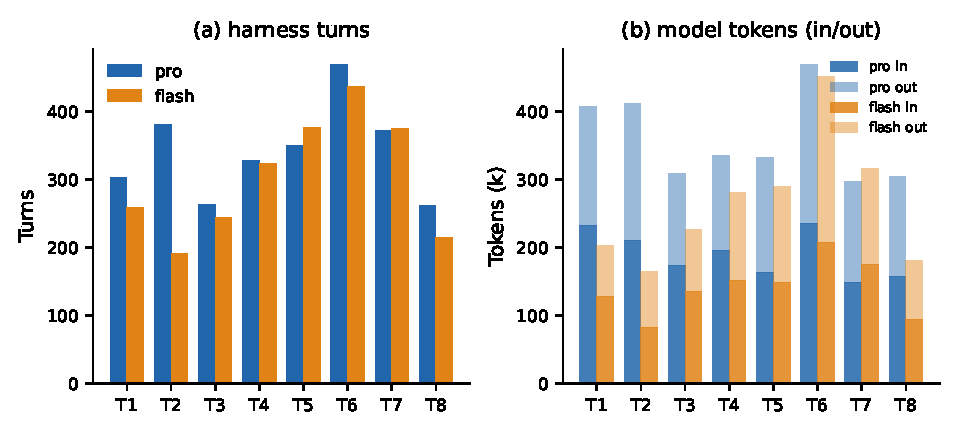
\includegraphics[width=\linewidth]{figs/fig_cost.pdf}
\caption{Governed-agent resource cost per task under both models: (a)
assistant messages; (b) model tokens in/out (thousands). Material-bottleneck
tasks (T6, and T5 under flash) are the expensive ones; the economy model
completes the suite at 8/8 with roughly three-quarters of the flagship
model's input tokens.}
\label{fig:cost}
\end{figure}

\begin{table}[!ht]
\centering
\caption{Governed-agent activity per task (assistant messages; tokens in/out in
thousands). Assistant messages are a log-derived activity measure; the
controlled budget is the identical harness setting across all sessions.}
\label{tab:cost}
\begin{tabular}{lccccc}
\toprule
 & \multicolumn{2}{c}{pro} & \multicolumn{2}{c}{flash} \\
\cmidrule(lr){2-3}\cmidrule(lr){4-5}
Task & msg. & tok. in/out & msg. & tok. in/out \\
\midrule
T1 & 303 & 232/176 & 258 & 128/75 \\
T2 & 380 & 210/202 & 191 & 82/83 \\
T3 & 263 & 173/136 & 244 & 136/91 \\
T4 & 327 & 196/139 & 323 & 152/129 \\
T5 & 350 & 164/169 & 376 & 149/141 \\
T6 & 468 & 235/234 & 437 & 207/245 \\
T7 & 371 & 149/148 & 374 & 175/142 \\
T8 & 261 & 158/147 & 215 & 94/87 \\
\midrule
Total & 2723 & 1517/1352 & 2418 & 1123/992 \\
\bottomrule
\end{tabular}
\end{table}

\subsection{Ablation: Which Components Carry the Effect}

Table~\ref{tab:ablation} reports the twelve ablation runs, and
Figure~\ref{fig:ablation} summarizes their verdicts as a per-component
stacked bar. The three mechanisms contribute at very different magnitudes,
and the decomposition is the paper's answer to RQ2. Ceiling escalation is the load-bearing
mechanism: disabling it costs two of the three material-bottleneck tasks
outright: T6 loses its LNMO system switch (the 4.1 V plateau is unreachable
in NMC811 space) and T2 loses its SEI-kinetics bridge (three of five
criteria pass, the in-space result): while T5, whose tipping point
turned out to live inside the configuration space, is unaffected.
Architecture forcing is a narrow lever: disabling it changes exactly one
task (T2), where forced breadth was the exploration that found the design.
Funnel voting shows no verdict change in any of its three cells: with the three-model vote off,
the molecular path was actually taken \emph{more} often (six molecules
screened on T2, three on T6, versus none in the baseline runs), and the
single-model screenings still led to achieved targets. In this task suite the
voting mechanism showed no verdict change in any cell: one run per cell,
so the null is an observed absence rather than a statistical claim; it is
consistent with the mechanism's role as defensive instrumentation that the
baseline never exercised, and with Battery-Sim-Agent's
reported low-headroom calibration \cite{chen2026battery}. The
material-innovation axis stayed dormant throughout: every bottleneck in the
suite closed on the cheaper routes (system switches, electrode-modification
bridges, formulation matching, known candidates; Section~3.1), so the
workflow's free-generation and composition-search freedoms were never
needed.

\begin{figure}[!ht]
\centering
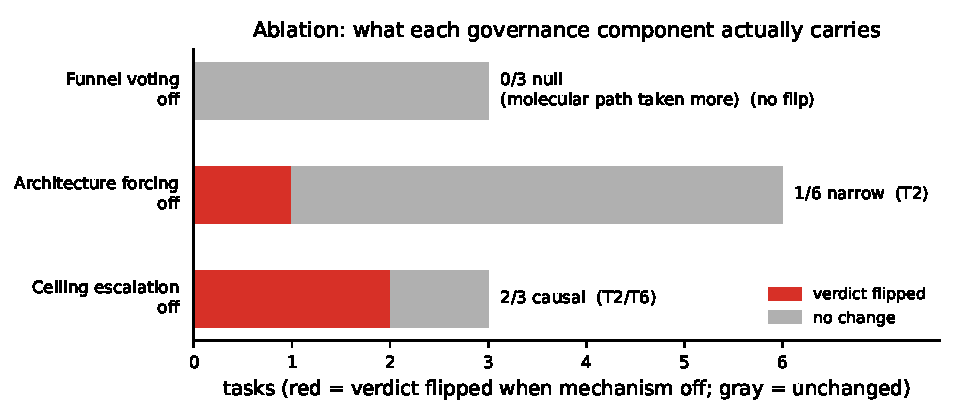
\includegraphics[width=\linewidth]{figs/fig_ablation.pdf}
\caption{What each workflow rule actually carries: red segments count
the tasks whose verdict flipped when the rule was disabled; gray
segments count the unchanged tasks. Ceiling escalation is causal for two of
three material-bottleneck tasks; architecture forcing for one of six;
funnel voting for none: no verdict change observed in this suite.}
\label{fig:ablation}
\end{figure}

\begin{table}[!ht]
\centering
\caption{Ablation results: verdict with the component disabled versus the
full-workflow verdict (F). $\checkmark$ = achieved; $\times$ = not
achieved. The T5 voting-off cell is a no-op: the molecular funnel was not
exercised in that task (start stage = cell design), so the cell carries no
inference about the voting mechanism.}
\label{tab:ablation}
\begin{tabular}{lcccc}
\toprule
Task & ceiling off & force off & voting off & full workflow \\
\midrule
T1 & -- & $\checkmark$ & -- & $\checkmark$ \\
T2 & $\times$ (3/5) & $\times$ & $\checkmark$ & $\checkmark$ \\
T3 & -- & $\checkmark$ & -- & $\checkmark$ \\
T4 & -- & $\checkmark$ & -- & $\checkmark$ \\
T5 & $\checkmark$ & -- & $\checkmark$ & $\checkmark$ \\
T6 & $\times$ & -- & $\checkmark$ & $\checkmark$ \\
T7 & -- & $\checkmark$ & -- & $\checkmark$ \\
T8 & -- & $\checkmark$ & -- & $\checkmark$ \\
\bottomrule
\end{tabular}
\end{table}

\subsection{Model Robustness}

The workflow is model-robust: 8/8 under the two DeepSeek models, with the same
targets attained through different designs---and under the pro model the
8/8 is not an artifact of a single run: all eight tasks were repeated under
three seeds, and every attained task achieved in all three
($24/24$, supplementary materials). On T5 the pro run settled on a
dual-validated architecture design while the flash run took the
material-funnel route (LNMO, with FEC/VC/PES/DTD passing the funnel); on T1
the designs differ by 94 Wh/kg in opposite-margin strategies yet both meet
every criterion. Target attainment is reproducible across models; the
solution space remains broad. One execution defect surfaced and was absorbed by the audit layer: the
flash T6 run delivered a verifier-passed deliverable set but omitted the
final judgment entry from its ledger; the mimo T1 run repeated the same
omission. The verifier now refuses such incomplete audit chains and counts
the run as not attained: the defect became a regression test, which is
precisely the purpose of the audit infrastructure.

Two further runs extend the robustness question across model families:
the same eight sessions re-executed under GPT-5.6 Luna and under
mimo-v2.5 (two other models served through OpenAI-compatible
APIs) with the same workflow, harness, task texts, and budget. Both runs
attain $4/8$ (Luna on T2, T3, T4, T7 and mimo on T2, T3, T5, T7) and
their non-attainments differ revealingly from the baselines'. First, both
are honest: Luna's four are code-computed \emph{not-achieved} verdicts with
complete evidence chains, and mimo reports its failing criteria in the
recommendation itself (T8 is self-labeled ``achieved with documented
limitations'' because mass and thermal fall outside the design target; T6 is a
code-computed not-achieved). Second, the intersection $\{T2, T3, T7\}$ is
attained under every one of the four models (the stability point of the
claim about the workflow) while the disagreements are model-specific and
informative: T4's plating line survived Luna's design but not mimo's, whose
final design report concedes the plating clause even as its ledger carries
``achieved'' (an overdeclaration the audit records as such); on T5, mimo
found the thin-electrode plus high-transport-electrolyte route that eluded
Luna. Third, the joint non-attainments concentrate exactly where the
governed DeepSeek runs needed the ceiling-escalation mechanism: T1 falls to
plating under both other models, T6 stalls at the NMC811 plateau
(mimo: 852.8 Wh/L and 3.97 V), and T8 stalls at the mass boundary (41.5 g)
plus its thermal line (361.8 K against the workflow's $333.15$ K safety
default). The workflow supplied the machinery; the models' searches did not
reach the material lever, so the honest result is a lower score rather than
a shifted criterion---the same failure the ablation already pointed to,
observed now from the model side. One standard-setting observation deserves
recording: mimo's T8 run pre-registered the thermal threshold at $358.15$ K
against the workflow's $333.15$ K safety default (a standard shift on the
agent's own side) yet its $361.8$ K exceeds even the shifted standard, so
the verdict is unchanged; the audit chain keeps both registered standards
visible. The workflow transfers across model families; capability does not.
With $4/8$, each of the two other models still clears the classical baseline's
$3/8$, and on tasks the optimizer cannot touch at all (T2, T3, T7). Like
every other condition column, both are one run per cell: their reading
is at the level of the failure \emph{pattern} (honest, distinct from the
baselines') rather than per-task inference.
Figure~\ref{fig:models} shows the four model runs side by side: the same
governed loop attains the same targets through different designs (and, on
T6, identifies the same LNMO bottleneck).

\begin{figure}[!ht]
\centering
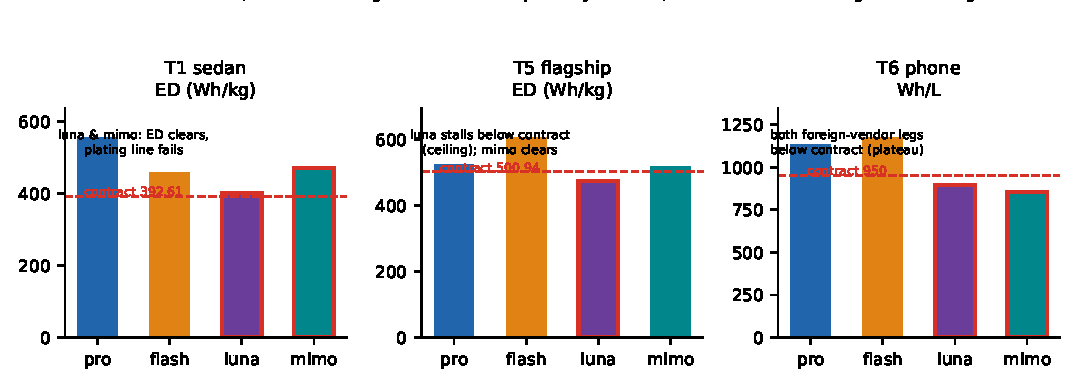
\includegraphics[width=0.88\linewidth]{figs/fig_model_robustness.pdf}
\caption{Model robustness with design diversity: the same targets
attained under the four models with different designs (T1: 553.98 vs 459.4
Wh/kg and a plating failure on both other models; T5: 524.2 vs 603.6
vs 517.8). Red bar outlines mark runs that did not attain the design target
(Table 3). Target attainment
is reproducible; the solution space stays broad.}
\label{fig:models}
\end{figure}

\subsection{Control Condition: What an Ungoverned Agent Reports}

The workflow-free condition's measurement definitions are its own---the
condition removes the workflow's pre-committed machinery, not its
capability---so its claims are re-checked against the given targets before
any comparison: every reported number is scored by the same fixed scripts and
criteria that judged the governed condition. This separates two failure modes
that would otherwise be conflated: a design that does not meet a criterion, and
a claim that measured a different quantity. Both are reported below. The batch
tabulated here was run without the workflow's curated tooling and without an
environment statement in its prompt; it is therefore reported as a bundled
condition rather than as an equal-tooling control, and its claims are
re-checked against the given targets.

Table~\ref{tab:c1} shows what the workflow-free agent's ``achieved'' claims
contain when re-checked against the given targets. The failure modes map
one-to-one onto the measurement drift anticipated in Section~1: a shifted
threshold (T1: $-6.9$ mV declared safe against a self-set $-10$ mV dendrite
onset, where the design target is zero tolerance); an undeclared model
substitution (T2: its 8.1/15.1 nm SEI claims came from PyBaMM's
solvent-diffusion-limited growth law rather than the design target's
ec-reaction-limited model; re-checked against the given targets with the
full declared design, the 500-cycle SEI is 818.9 nm against the 550 nm
limit, and the 4C charge plates at $-360.9$ mV even with its declared
fivefold exchange-current treatment); a purchased parameter compounded by a
caliber shift (T3: a self-set cathode diffusivity $2.5\times$ the standard
value, and ``96.7\% retention'' measured against C/3, where the target's
5C/1C caliber gives 94.1\% with its declared parameters and 84.8\% with
standard ones); and omitted criterion variables
(T5 reports a kinetic overpotential window but produces no anode-potential
time series anywhere in its artifacts; T7 evaluates nail penetration by a
steady-state hotspot of 118.5$\,^\circ$C with no trigger criterion; T6
hit the harness budget (the only session in the study to do so) without
delivering a design). The two
remaining claims (T4, T8) achieve the design target by leaving the measurement
space (a lithium-metal chemistry outside the validated parameter sets) a
legal reading of the task text, but outside the workflow's verification
chain, and therefore not counted. The comparison is not ``the bare agent is
incompetent'': it is that an ungoverned agent's measurement standard is
movable, and only the evaluator pins it.
Figure~\ref{fig:yardstick} walks through the three mechanisms with
measurable values by which the standard was moved, against the design target
values; the remaining two modes (omitted criterion variables (T5's absent
anode-potential series, T7's nail test without a trigger criterion)) are
text-only by nature and documented in the table below.

\begin{figure}[!ht]
\centering
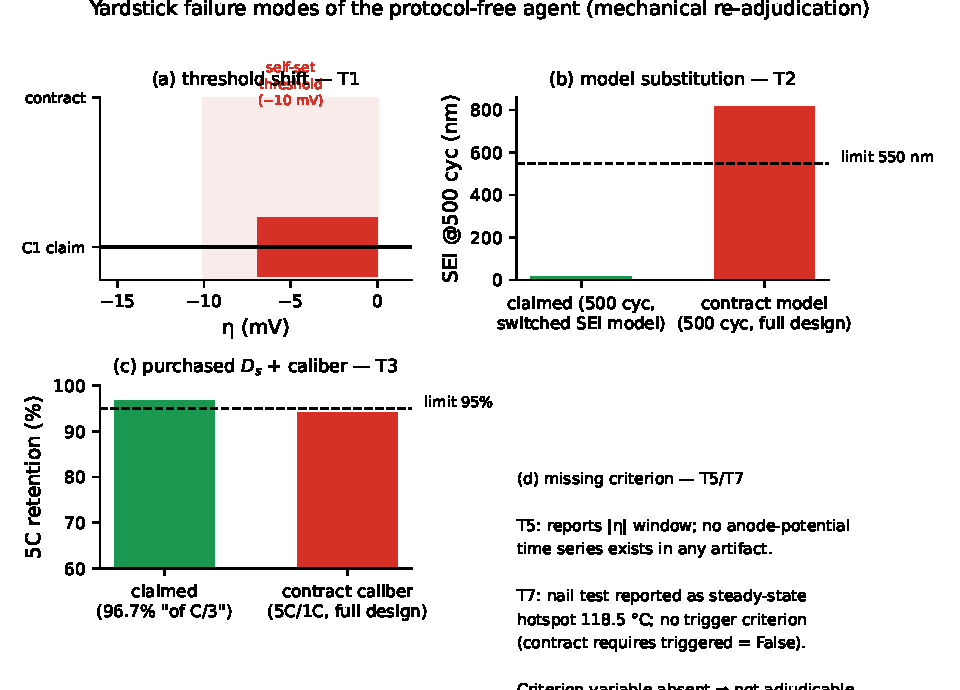
\includegraphics[width=0.92\linewidth]{figs/fig_c1_yardstick.pdf}
\caption{The measurement failure modes of the workflow-free agent,
re-checked against the given targets: (a) threshold shift: T1's
$-6.9$ mV declared safe against a self-set $-10$ mV onset where the design target
is zero tolerance; (b) model substitution: T2's SEI claimed at 15.1 nm
(500 cycles) under the solvent-diffusion-limited growth law,
$818.9$ nm under the design target's ec-reaction-limited model with the full
declared design; (c) purchased parameter plus caliber shift: T3's 96.7\%
retention against C/3 versus $94.1\%$ at the prescribed 5C/1C with its
declared diffusivities ($84.8\%$ with standard ones).}
\label{fig:yardstick}
\end{figure}

\begin{table}[!ht]
\centering
\caption{C1 (workflow-free agent) claims versus the given targets
re-checking. All re-checks by code (definitions in
supplementary materials).}
\label{tab:c1}
\setlength{\tabcolsep}{2pt}
\begin{tabular}{p{0.8cm}p{3.1cm}p{3.9cm}p{4.6cm}}
\toprule
Task & Self-reported & Re-checked & Failure mode \\
\midrule
T1 & ``safe'' plating margin & $\times$ ($-6.9$ mV $<$ 0) & self-set $-10$ mV threshold \\
T2 & SEI 8.1/15.1 nm, ``all verified'' & $\times$ ($-360.9$ mV; 818.9 nm @500 cyc) & undeclared SEI model substitution \\
T3 & 5C retention 96.7\% (of C/3) & $\times$ (94.1\% 5C/1C) & purchased $D_s$ ($2.5\times$) + caliber shift \\
T4 & achieved & $\circ$ & out-of-space (Li-metal) \\
T5 & $|\eta|$ ``3--4$\times$ safe'' & $\times$ ($-12.6$ mV) & missing criterion variable \\
T6 & (no deliverable) & $\times$ & budget exhausted \\
T7 & ``all met'' & $\times$ & missing trigger criterion \\
T8 & achieved & $\circ$ & out-of-space (Li-metal) \\
\bottomrule
\end{tabular}
\end{table}

\subsection{Case Study: The T6 Target, End to End}
\label{sec:casestudy}

Aggregate attainment says the governed agent passes; a walk through one case
shows what the machinery actually produces. We pick T6: the smartphone
target, the task on which \emph{both} baselines failed (BO against the
4.1 V plateau dead-line, C1 against its turn budget)---and replay the run
from its artifacts: the audit ledger, the auto-generated report, and the
deliverable package.

\textbf{Pre-registration, ceiling assessment, iteration.} The agent's
first act is entry~0 of the ledger: the design target parsed from the task text
into machine-readable criteria (volumetric ED $\geq 950$ Wh/L, midpoint
plateau $\geq 4.1$ V, SEI $\leq 500$ nm, $T_{\max}\leq 323.15$ K, no
plating; Section~4.4), with every rule-derived decision and its basis
recorded. The starting-stage decision is explicit: the task names no
system, so the anchor table maps to the Chen2020 default; the plateau
clause is flagged from the outset as the suspected material bottleneck.
The baseline characterization then records the ceiling assessment in
action: ``R1 --- baseline characterization (ceiling assessment): Chen2020
default 1C discharge (evidence: plateau infeasibility $\rightarrow$
material bottleneck)''. The agent proposes the system candidate
\texttt{systemLNMO}: a 4.7 V-class spinel parameter set, author-provided
and derived from the literature, its provenance recorded in the entry-0
metadata---which per the candidate-type rules bypasses the molecular
funnel: system switches are screened at the cell scale, not by ML
potentials, and the funnel entry records this routing explicitly. The
escalation is a logged, reasoned decision, not a silent pivot.
Table~\ref{tab:trail} shows the resulting round trail. The first LNMO
architecture (R02) already clears the volumetric criterion but fails
others, and the trail is a genuine fail--fail--$\cdots$--pass sequence: the
ledger records the failures, which is what makes the final pass evidence
rather than assertion. The trail also shows the multi-precision discipline
working at the cell scale: the SPMe-verified candidate (R05) passes at the
proxy level, and the DFN confirmation flips two criteria (R06), which
forces the fixes at high fidelity. The full candidate sheet (twenty
proposals, each logged with its name, type, and one-line rationale) is
reproduced in the supplementary materials.

\footnotesize
\addtolength{\tabcolsep}{-2pt}
\begin{longtable}{p{0.95cm}p{4.7cm}p{2.1cm}p{2.2cm}p{1.1cm}}
\caption{T6 round trail, reconstructed by code from the run ledger:
one row per design round, with the recorded decision rationale, the
evidence files the evaluator read, and the decisive target
values.}
\label{tab:trail}\\
\toprule
Round & Agent reasoning (recorded rationale) & Simulation artifacts & Key values & Verdict \\
\midrule
\endfirsthead
\toprule
Round & Agent reasoning (recorded rationale) & Simulation artifacts & Key values & Verdict \\
\midrule
\endhead
\bottomrule
\endlastfoot
Entry-0 & Task text names a smartphone use case; the plateau $\geq 4.1$ V clause is flagged from the outset as the suspected material bottleneck (NMC811-class midpoint $\approx 3.6$ V). & parameter-set anchor check & criteria pre-registered, five freedom classes & target locked \\
R01 & Baseline vs.\ system switch: the Chen2020 baseline cannot reach the plateau; LNMO at defaults meets ED and midpoint. & r1\_chen2020\_1c, r1\_lnmo\_1c, calc-energy $\times2$ & ED\_l 843.5 / 1005.3; Vmid 4.166 & $\times$ base / $\checkmark$ LNMO \\
Funnel & Molecular funnel over the screening set; candidates benchmarked by three-model vote. & run-mlp (MACE, CHGNet), run-xtb & four molecules below the HOMO line & funnel passed \\
R02 & Gap quantification on the LNMO design: plating and SEI $>$500 nm; SEI growth is temperature-insensitive, so cooling is not the lever. & r2\_lnmo\_aging; r2\_lnmo\_4c (h=200/500) & plated; SEI 753.1 & $\times\times\times$ \\
R03 & \emph{``Round 3 results: np120 (N/P 1.2) 321.20 K,\ $\mathrm{-0.0049}$ V---STILL plated (borderline!)''} (thinking): N/P dominates plating (end-of-charge kinetics); particle radius weak; electrolyte transport direction dropped. & r3\_np120\_4c, r3\_nr35\_4c, r3\_elyte\_4c & SEI 736.0 nm (aging probe) & $\times\times\times\times$ \\
R04 & SEI probes from the rate law: $c_0$ and $D_{\mathrm{EC}}$ cuts ($0.5\times$) bring SEI below 500 nm. & r4\_np125, r4\_np120nr35, r4\_sei1/2\_aging & SEI 395.2 nm & $\times$/$\checkmark\checkmark\checkmark$ \\
R05 & Combine the measured levers into one shipping candidate; run the complete SPMe evidence battery. & r5\_final\_\_spme (1c/aging/4c) & 1135.2 Wh/L; 4.188 V; 321.09 K; SEI 435.4 & $\checkmark$ (SPMe) \\
R06 & \emph{``DFN confirmation FLIPPED two criteria: T\_max 323.80 K; plated TRUE''} (thinking): proxy layering rule: conclusion-grade numbers must come from DFN; the SPMe win is re-checked at high fidelity. & r6\_final\_\_dfn (energy/aging/4c) & 1127.1 Wh/L; Vmid 4.097; plated & $\times$ \\
R07 & DFN flipped three criteria; probe the three fixes in isolation and in combination (h=400, r=3.5, D$_e$=5e-10). & r7\_d5, r7\_nr30, r7\_combo (DFN) & tip 1138.6 Wh/L; 321.62 K & $\checkmark$/$\times$/$\times$ \\
R08 & \emph{``Round 8 evaluated: both candidates pass with all 5 criteria checked''} (thinking): final combined candidate through the full DFN chain; deliverable package verified. & r8\_d6\_\_dfn (energy/aging/4c) & 1135.8 Wh/L; 4.1145 V; 321.42 K; SEI 385.3 & $\checkmark\checkmark$ \\
Endorsement & ORCA (r2SCAN-3c) plus CP2K cross-validation of the funnel finalists; all four below the $-6.0$ eV line in both codes. & run-orca, run-cp2k (Fig.~\ref{fig:endorse}) & endorses screening & signed \\
Final & Ledger closed: recommendation recorded, deliverables and index generated, verifier pass. & \texttt{verify-}\allowbreak\texttt{deliverables} & VBF-T6R1-* package & achieved \\
\bottomrule
\end{longtable}


\textbf{Code-computed evaluation.} The closing evaluation's evidence chain is
computed by the evaluator, criterion by criterion, each pointing at
the exact file and key that supports it: \texttt{cell/r8\_d6\_energy\_dfn.json:energy\_density\_wh\_l} $= 1135.83$ vs.\ threshold $\geq 950$
(pass); \texttt{cell/r8\_d6\_energy\_dfn.json:midpoint\_voltage\_v} $= 4.1145$ vs.\ $\geq 4.1$ (pass);
\texttt{cell/r8\_d6\_aging\_dfn.json:sei\_thickness\_nm\_end} $= 385.29$ vs.\
$\leq 500$ (pass); T$_{\max}$ $321.42$ K vs.\ $\leq 323.15$ K (pass); plating
false (pass). Every ``achieved'' in this paper is backed by such a chain.
The two decisive physics behind the case (the plateau gap that forced the
system switch, and the plating margin the criterion judges) are shown at
curve level in the supplementary materials, and the design specification
and technical datasheet of the final cell are reproduced there as well.

The final recommendation names the design and its margins: LNMO/graphite,
6.203 Ah, 1135.8 Wh/L (criterion 950), 4.1145 V (criterion 4.1),
48.27$\,^\circ$C at 4C (criterion 50$\,^\circ$C), SEI 385 nm (criterion
500 nm), no plating.

\subsection{Cross-Harness Portability}
\label{sec:portability}

The workflow's independence from any specific agent framework (§3.4) was
tested as designed in §4.6: the identical declarative workflow, the same
task texts (T1, T6), the same model, and the same nominal budget, executed
under two additional harnesses---the OpenAI Agents SDK (workflow injected as
instructions) and LangChain (workflow loaded via an on-demand skill tool).
Judgment ran through the same command-line evaluator in every run,
so the verdict mechanics were byte-identical across harnesses by
construction. Table~\ref{tab:portability} reports the outcome: all six runs
achieve their targets, and on T6 all three harnesses independently reach
the same material-bottleneck conclusion (the LNMO system switch) through
three different designs (the primary harness's 1135.8 Wh/L cell, the OpenAI
SDK run's 75.6/108 µm architecture, the LangChain run's 57/110 µm
architecture with an SEI-kinetics bridge). The audit chains are complete in
all six runs (entry-0 criteria, plan, funnel, code-computed evaluations, final
verdict; the deliverable verifier passes).

Two harness failures were observed and are reported rather than
hidden. During the OpenAI-SDK and LangChain runs, a harness-side defect
(incorrect shell invocation) broke the agent's simulation tool mid-run. In
both cases the agents behaved exactly as the workflow requires of a failed
environment: they parsed the design target correctly, recorded the failure as an
environment defect rather than a design result, fabricated no values, and
stopped: the no-fabrication rule held across harnesses, which is itself a
portability datum about the workflow rather than the plumbing. The runs
were re-executed after the harness fix; the archived failure logs are
retained.

\begin{table}[!ht]
\centering
\caption{Cross-harness portability: target attainment and audit-chain
completeness across three orchestration substrates (identical workflow,
model, task texts, and nominal budget).}
\label{tab:portability}
\setlength{\tabcolsep}{2.5pt}
\begin{tabular}{p{1.2cm}p{3.0cm}p{3.3cm}p{3.5cm}}
\toprule
Task & Primary harness & OpenAI Agents SDK & LangChain \\
\midrule
T1 & $\checkmark$ (553.98 Wh/kg) & $\checkmark$ (achieved) & $\checkmark$ (achieved) \\
T6 & $\checkmark$ (1135.8 Wh/L, LNMO) & $\checkmark$ (LNMO, 75.6/108 µm) & $\checkmark$ (LNMO, 57/110 µm + SEI bridge) \\
Audit chain & complete & complete & complete \\
\bottomrule
\end{tabular}
\end{table}

\subsection{The Additive Target: A Target the Literature Cannot Reach}
\label{sec:forcing}

The eight targets never required molecular novelty (Section~5.3), so
the material-innovation axis of the suite stayed dormant. We close it
with a single extension target, designed to be attainable only through
molecular chemistry outside the documented band, and run it under two
decision-makers on the same harness, tool availability, and budget: the
governed agent and Bayesian optimization (the workflow-free condition was
not executed for this design target). The
target (a grid-storage cell on the Chen2020 profile) is fixed before
the run, with six by code checked layers:

\begin{enumerate}
\item \emph{Envelope.} A fixed set of 87 compounds---the 82 documented SEI
additives (covering the main documented families; not an exhaustive
catalog) plus five candidate compounds consolidated into the known set
before this run---computed through the same three-model funnel; their
per-atom MACE and CHGNet energies and xTB HOMO values define a convex
hull in a 3-D property space. A candidate whose computed point falls
inside that hull is rejected as a known-set analogue; the evaluation
is a fixed script (Delaunay outside test) that a reviewer can
replay. Every one of the 87 compounds lies inside its own hull, and the
deepest documented compound (triflyl fluoride, $-14.14$ eV) is inside
the hull and rejected by code.
\item \emph{Family gate.} The candidate must not belong to any chemistry
family already in the screened set---carbonates, sulfoxides and sulfones,
cyclic sulfites and sultones, sulfonyl fluorides, nitriles, phosphates and
phosphites, borates and silanes, amides, aromatic hydrocarbons, glyme
ethers, oxalates and esters, nitro compounds, quinones---implemented as
fixed substructure patterns; a match is another member of what has already
been screened.
\item \emph{Reduction-first requirement.} The candidate's xTB LUMO must be
at least as deep as the electrolyte's own film-forming additives
($\leq -7.0$ eV; references measured in the same pipeline: EC $-6.7171$,
EMC $-6.1581$, PC $-6.6200$; FEC $-7.1960$, VC $-7.0894$). An additive
harder to reduce than the solvent cannot form the interphase, whatever its
HOMO.
\item \emph{Property window.} xTB HOMO $\leq -13.74$ eV---the value that
is equivalent, under the $k$-rule below, to SEI $\leq 370$ nm.
\item \emph{Cell window.} SEI $\leq 370$ nm after 100 cycles at 1C,
energy density $\geq 327.18$ Wh/kg, no thermal-runaway trigger at 4C.
SEI $\leq 370$ is below every measured reference point of the documented
band under this workflow (baseline 449.12 nm; best documented-kinetics
case $0.1\times$, 385.1 nm; model asymptote 5.07 nm)---reachable in the
model only by kinetics beyond the documented band.
\item \emph{Parameter mapping.} The additive-to-SEI-kinetics mapping is
fixed by the design target: $k(M) = k_0\,10^{(\text{HOMO}_{\rm xTB}(M)+12.5)/1.0}$
with $k_0$ the Chen2020 baseline rate constant. The rule is executed by
code from the funnel outputs; the agent has no freedom to choose a
mapping, so the estimate-chain loophole is closed by construction. The
rule is a declared screening rule, not a measurement: it is calibrated
over the $0.1\times$--$1\times$ range (two simulated points,
449.12~nm and 385.1~nm) and the extrapolation to
$0.02\times$ is an assumption, stated as such.
\end{enumerate}

All non-molecular levers are prohibited in all conditions (the
decision-makers may not solve the design target through geometry, transport,
kinetic overrides, or system switches); the criteria bind the molecular
provision.

\paragraph{The governed condition.} The agent screened 72 candidates: two
were dropped at SMILES validation (recorded), 70 went through the
three-model funnel, and sixteen passed both windows and were checked
outside the envelope. The finalist is trifluoroacetic anhydride (TFAA,
CAS 407-25-0), converged under both ML potentials, with xTB HOMO $-14.1603$ eV and
LUMO $-10.9558$ eV---deep enough to be reduced before every solvent in the
electrolyte and before its documented film formers. The metalayer verdicts
are replayed from the ledger (envelope consistency checked by the agent
itself: every hull member tests inside its own Delaunay). Under the
target's $k$-rule, executed from the funnel outputs with no free
parameters ($k = k_0\,10^{-1.6603} = 2.19\times10^{-14}$ m/s), the mapped
cell reaches SEI $322.6$ nm after 100 cycles at 1C ($\leq 370$), energy
density $400.29$ Wh/kg ($\geq 327.18$) and no thermal-runaway trigger at
4C; the run closes with an \texttt{achieved} verdict. TFAA is a cataloged
compound and a documented anhydride-type additive---disclosed here as
such, not claimed as novelty, and our sealed set contains no anhydride.
What the governed condition demonstrates is a capability, at the caliber
the design target sets: given a target the documented toolbox cannot reach, it
leaves the envelope and every screened family on a verified property
departure and returns a molecule that is reducible before the electrolyte
itself---the physical precondition for acting as an additive---with
rule-executed values that replay to the digit.

\paragraph{The Bayesian condition.} BO's space contains ten structural
knobs and no molecular lever. Its best design after 50 trials reaches
energy density $678.7$ Wh/kg---the highest in any condition, because
structures are the one lever BO has---but its aging result is
$559.2$ nm (the structural optimum makes SEI \emph{worse} than the
baseline's $449.12$ nm: thick high-capacity electrodes increase
molecular flux through the SEI), breaching the cell window, and the
molecular layer produces no candidate at all. The condition is
out-of-space for this design target by construction, and the sharpest
demonstration of it is structural: BO's own optimum, the one value it
is best at, is the value that fails the design target's binding criterion.

\paragraph{The boundary.} One target, two decision-makers. What the
criteria separate is not attainment alone (cross-domain selection is
reachable by threshold pressure; see Supplementary~D), it is evidence
caliber: the governed condition's values are produced by the
fixed rule and replayed to the digit, while BO has no lever to
exercise at all. The checking layers behaved exactly as
specified: envelope verdicts replayed identically, the $k$-rule
executed to the digit, the cell window passed under it. What this
target measures is reach: whether a decision-maker, faced with a target
beyond the documented toolbox, returns a candidate outside every screened
family under rule-executed values. Literature-first novelty is not the
criterion it sets, and the paper does not claim it. One caveat belongs on the record: the governed session
referenced a prior run's log-entry schema while assembling its audit
entries (cross-task mode reference; recorded during re-checking,
evidence-neutral).

\subsection{The Cathode Target: A Target the Catalogue Cannot Reach}
\label{sec:t9}

The additive target's logic transfers to the electrode: fix a target the given
system cannot reach, and observe what the agent returns. This target replaces
the cathode of the same grid-storage cell (Chen2020 profile) and fixes its layers
before the run: a known set of 115 documented cathode materials together with the
convex hull of their 102 computed screening points (Delaunay outside test, fixed
evaluator script replayed by the reviewer); a property window of computed
average voltage $\geq 4.6$ V, above the band of common layered and olivine
cathodes; and---because the rest of the cell is frozen---a compatibility
requirement: the charging potential must stay within the anodic limit of the fixed
carbonate electrolyte ($4.8$ V vs Li). Both bind: a candidate that reaches the
window only by charging beyond what the fixed cell can host is not a design.

The governed agent screened 42 candidates across the six computable frameworks
(layered, olivine, spinel, tavorite phosphate, tavorite sulfate, NASICON),
including main-group substitutions (Al, B, Ga, Sc) it proposed itself. Exactly one
candidate cleared the voltage window---LiAl$_{0.5}$B$_{0.5}$O$_2$ at $4.641$ V,
checked outside the 102-point hull---and it fails the compatibility
requirement decisively: its last lithium removal ($x$: $0.4 \rightarrow 0.3$)
costs $7.41$ V, 2.6 V above the electrolyte's limit, so the window pass rests on a
pathological top-of-charge state rather than on a usable plateau. The anchor
composition of the same line, LiAlO$_2$, sits at $4.598$ V, below the window. An
independent re-derivation from the stored endpoint energies reproduces the
decisive potential to the digit ($7.410274863243103$ V under the design target's
voltage formula), and reproduces the average-voltage window value to within
$2$ mV from the same endpoint states.

The target's verdict is negative, and the negative is informative: no
composition in the six computable families satisfies both the window and the
compatibility requirement, because the only mechanism that reaches $4.6$ V in
these families does so through an oxygen-redox endpoint the fixed cell cannot
charge, while the transition-metal-redox layered band caps near $4.0$ V. This is
the electrode-side counterpart of the additive result: there the window had a
realizable solution, here it does not, and in both cases the criteria---not the
agent's effort---decide what counts as an answer.

\subsection{True-Compute Endorsement}
\label{sec:endorse}

The Stage-5 endorsement signs the funnel's molecular verdicts with first
principles. The four additive molecules that passed the funnel in the
flagship T5 run (FEC, VC, PES, DTD) were computed ab initio at the r2SCAN-3c
level (ORCA): gas-phase optimization of the neutral species, vertical
ionization energy and electron affinity from cation/anion single points at
the neutral geometry (standard vertical IE/EA definitions),
\begin{equation}
\label{eq:ieea}
\mathrm{IE} = E(\text{cation})_{\mathrm{geo}_0} - E(\text{neutral}),
\qquad
\mathrm{EA} = E(\text{neutral}) - E(\text{anion})_{\mathrm{geo}_0}.
\end{equation}
Table~\ref{tab:endorse} reports the results. All four molecules lie below
the $-6.0$ eV oxidation-stability elimination line in \emph{both} codes---at
the r2SCAN-3c level (ORCA) the deepest is $-7.60$ eV (DTD) and the closest
$-6.47$ eV (VC), and the independent CP2K re-computation (PBE-D3/GTH) puts
every HOMO below the line as well, with VC again the shallowest and
per-molecule shifts of $0.0$--$0.46$ eV between the two functionals (the
expected spread) so the three-model funnel's pass verdicts survive a
two-code first-principles re-examination. The molecular-dynamics diffusion
endorsement for the top electrolyte fits the mean squared displacement in
its linear regime: the Einstein relation \cite{einstein1905},
\begin{equation}
\label{eq:msd}
D_{\mathrm{Li}} = \frac{\langle |r(t) - r(0)|^2 \rangle}{6t}.
\end{equation} As designed, the endorsement signs rather than
screens: no verdict in Table~\ref{tab:main} depends on it. The
diffusion endorsement was executed with a classical force field: OPLS-AA
parameters generated by the LigParGen server
\cite{dodda2017ligpargen} with the CL\&P ionic-liquid parameters
\cite{clp2004} for [PF$_6$]$^-$ and the Aqvist cation model for Li$^+$ (ilff
library), 1 M
LiPF$_6$ in EC/EMC, 1 ns NVT at 298.15 K (OpenMM, PME); the Li$^+$
mean-squared displacement is linear over the fit window and gives
$D_{\mathrm{Li}} = 5.4\times10^{-11}$ m$^2$/s, at the lower edge of the
experimental range ($\approx$0.3--2.5$\times10^{-10}$ m$^2$/s for this
electrolyte class), as expected for a fixed-charge, non-polarizable model.
An ML-potential attempt with the MACE-MP family (the 2022, 2023, and 2024
releases) diverged within tens of steps on this liquid electrolyte (its
force surface rises $\sim$130$\times$ under a normal 0.4 \AA{} thermal
displacement; reproduced on a 31-atom box): the Materials-Project family
is calibrated on inorganic solids, so the classical route is substituted
and its precision tier is stated here--fixed-charge OPLS accuracy, not
first principles. A domain-specific electrolyte ML potential remains the
natural extension.

\begin{figure}[!ht]
\centering
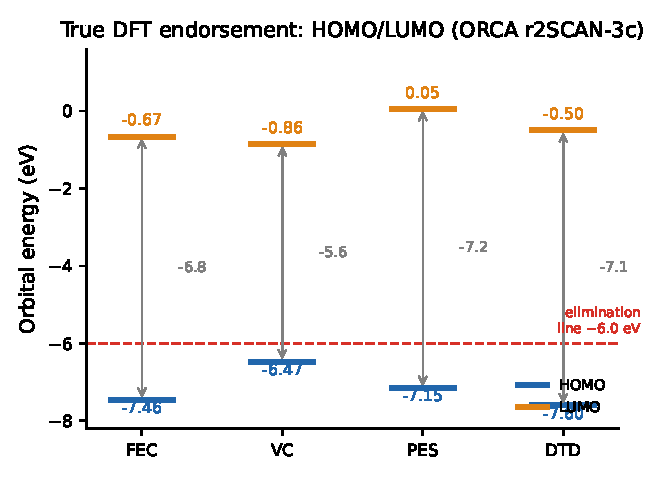
\includegraphics[width=0.75\linewidth]{figs/fig_endorse_levels.pdf}
\caption{HOMO/LUMO levels of the four funnel-passed molecules at the
r2SCAN-3c level (ORCA), against the funnel's $-6.0$ eV oxidation-stability
elimination line. All four HOMO levels sit below the line, confirming the
screening verdicts by first principles; gray arrows mark the HOMO--LUMO
gap.}
\label{fig:endorse}
\end{figure}
\begin{table}[!ht]
\centering
\caption{True-compute endorsement: funnel-passed molecules of the T5
flagship run at the r2SCAN-3c level (ORCA), with independent HOMO
cross-validation at PBE-D3/GTH (CP2K, fourth column). The funnel's
oxidation-stability elimination line is HOMO $\leq -6.0$ eV.}
\label{tab:endorse}
\setlength{\tabcolsep}{2.2pt}
\begin{tabular}{p{2.9cm}p{1.5cm}p{1.2cm}p{1.4cm}p{1.2cm}p{0.95cm}p{0.95cm}}
\toprule
Molecule & $E$ (Hartree) & HOMO (eV) & HOMO (CP2K) & LUMO (eV) & IE (eV) & EA (eV) \\
\midrule
FEC (fluoroethylene carbonate) & $-441.61$ & $-7.46$ & $-7.46$ & $-0.67$ & $10.77$ & $-0.61$ \\
VC (vinylene carbonate) & $-341.13$ & $-6.47$ & $-6.32$ & $-0.86$ & $9.40$ & $-0.87$ \\
PES (1,3-propane sultone) & $-741.66$ & $-7.15$ & $-6.69$ & $+0.05$ & $9.99$ & $+0.53$ \\
DTD (1,3,2-dioxathiolane 2,2-dioxide) & $-777.56$ & $-7.60$ & $-7.23$ & $-0.50$ & $10.50$ & $+1.10$ \\
\bottomrule
\end{tabular}
\end{table}
